\documentclass[a4paper,12pt]{article}

% Load Packages
\usepackage{amsfonts,amsthm,amsopn}
\usepackage[psamsfonts]{amssymb}
\usepackage[cmex10]{amsmath}
\usepackage{amsmath}
\usepackage{enumitem}
\usepackage{natbib}
\usepackage[left=3cm,right=3cm,top=2.5cm,bottom=3cm]{geometry}
\usepackage[dvipsnames]{xcolor}
\usepackage[]{graphicx}
\usepackage{graphics}
\usepackage[bb=dsserif]{mathalpha}
\usepackage{bm}
\usepackage{subcaption}
\usepackage{booktabs}
\usepackage{rotating,tabularx}
\usepackage[font=small]{caption}
\usepackage{ulem}
\usepackage{floatrow}
% Table float box with bottom caption, box width adjusted to content
\newfloatcommand{capbtabbox}{table}[][\FBwidth]

\newcommand{\ex}{\mathbb{E}} % expectation
\newcommand{\ind}{\mathbb{1}}
\newcommand{\bfbeta}{\bm{\beta}} %bold beta coefficent
\newcommand{\reference}[1]{\textcolor{black}{#1}}

\setlength\parindent{0pt}
\renewcommand{\baselinestretch}{1.2}

%\usepackage{xr}
%\externaldocument{../paper/paper}
%\externaldocument{../paper/supplement}
\usepackage{hyperref}

% Start document
\begin{document}



\begin{center}
\underline{\Large\textbf{{Reply to reports on article JBES-P-2022-0567.R1}}}\end{center}
\vspace{10pt}


First of all, we would like to once more thank the editor, the associate editor and the reviewers for their thoughtful comments and suggestions which have greatly helped to improve the paper. In the revision, we have addressed all points raised. Please see our point-by-point responses below. 
%While we incorporated as much new material as possible into the main text, some content (particularly from the revised simulation study) has still been allotted to the Supplement to meet the 35-page limit. We are happy to adjust the placement of content further if needed.

%We fully with referee 1 that the simulation study is an intergal part of the analysis of our methods and as such should be incorporated in the main body of the paper. However, toigether with all the new simulation exercises that we added in this revision round, the simulation study is now ?? pages in length. Given the 35-page-limit, we simply did not see how to do so and also thought that it is not very reader-friendly to put only parts of the simulations, parts of the theory in the paper but to keep them together. We hope this is understandle. 

%Please also note that we have tried to add as much of the new material as possible to the main body of the paper. However, to meet the 35-pages-limit, we still had to leave parts of the material . %, in particular, the revised simulation study (which comprises many additional simulation exercises) to the Supplement.
%If required, we can of course rearrange the material, shifting part of the simulations to the main body of the text while moving other parts to the Supplement. 



\subsection*{Reply to the associate editor}


\begin{enumerate}[label=\arabic*.,leftmargin=0.6cm]


\item {\color{black}\textit{(a) My apologies, but I maintain that your $H_0$ (page 3) is unnatural and uninteresting. In the trend analysis of multiple time series, it is extremely unlikely that the natural ‘position of ignorance’ is that all trend curves are the same. What if, for example, I already know or suspect that the curves form distinct groups? It is then something of a wasted effort to start from the position that they do not differ at all. \\
(b) Also, the null hypothesis is not robust to high-dimensionality as it is more likely that some curves will differ as I observe a higher number of variates (I understand that you do not do this in the paper but this only makes it even less interesting, in my view). \\
(c) As a cartoon illustration of the first point above, if I suspect that $p-1$ (say) curves may be the same, but 1 is distinctly different, do I need to first remove the offending one before performing your test, in which case I enter the territory of post-selection inference (which you do not cover), or do I not need to remove the offending one, in which case I am pretending that my $H_0$ is different from what it is in reality?}}

(a) We fully agree with you that -- as you put it -- our global null hypothesis $H_0$ ("all trends are exactly the same") is unnatural and uninteresting. In most applications, it is rather obvious that not all trends are the same. Hence, there is no need to formally test the hypothesis $H_0$ just to get the unsurprising answer that it is violated. However, it is very interesting and practically relevant (at least in our point of view) to understand in which ways $H_0$ is violated: which trends are different, in which time periods the trends differ, whether there are groups of (more or less) identical trends, etc. The main contribution of our paper is to develop statistical methods which provide this very relevant information. Specifically, we develop
\begin{enumerate}[label=(\roman*),itemsep=0pt,topsep=0pt,leftmargin=1.5cm]
\item methods to make simultaneous confidence statements about which trends are different and where (i.e., in which time intervals) they differ from each other 
\item clustering methods for finding groups of time trends (which come with certain statistical confidence guarantees). 
\end{enumerate}
We develop these methods in the context of a classical statistical testing framework. In this framework, the global null hypothesis $H_0$ appears as an auxiliary construct/concept which, however, is not interesting by itself but only a means to formally write up the methods/theory. \\
%Comparison to structural break tests:
%The situation is not unlike in change point analysis. Suppose we observe a time series  $\{ Y_t: t=1,2,\ldots \}$ and are interested in the time series of means $\mu_t = ex[Y_t]$. 
In summary, your criticism doubtlessly applies to standard tests of $H_0$ which only allow to say (with a certain statistical confidence) whether $H_0$ is violated or not, and which are thus very uninformative. However, it does not apply to our approach. Rather, our approach can be regarded as  -- at least a partial -- answer to your criticism of standard uninformative tests of $H_0$. In the introduction of the paper, we have emphasized this crucial difference between our approach and standard tests of $H_0$ as clearly as possible. 

(b) This is a fair point. A high-dimensional extension would indeed be very interesting. However, adapting the theory would be highly non-trivial, which is why we have not tackled this extension in the paper. 

(c) Simply run our methods on all $p$ curves. Then (if your guess is correct, i.e., if all curves are the same except for one), our methods will give you the following information (provided that the regularity conditions of our theory are satisfied): 
\begin{itemize}[itemsep=0pt,topsep=0pt,leftmargin=1.5cm]
\item (Asymptotically with probability $1-\alpha$) our inference methods will tell you (i) that all trends are the same except for one and (ii) in which time intervals this trend differs from the others. 
\item (Again asymptotically with probability $1-\alpha$), the clustering algorithm will give you two groups: a cluster with the $p-1$ identical trends and a singleton cluster with the other trend. 
\end{itemize}
Note that in the simulation study, we have used precisely such a cartoon setting with $p-1$ identical trends and $1$ different trend to showcase the power properties of our inference methods. 

%We appreciate your perspective regarding the null hypothesis $H_0$. We recognize that assuming identical trends across time series can seem restrictive in many real-world applications. However, we argue that our choice of $H_0$ is methodologically justified because it represents the simplest, most parsimonious starting point for testing. This aligns with the traditional Neyman-Pearson framework where the null serves as a benchmark for detecting departures. Furthermore, our multiscale method enhances this approach by not only rejecting $H_0$ but also identifying specific intervals and pairs of series where differences occur, providing actionable insights beyond a binary rejection decision. 

%%Furthermore, we understand your concerns about the robustness of $H_0$ in high-dimensional settings, where differences between some trends become more likely. However, our test is designed in a way that it controls family-wise error rate (FWER) irrespective of the number of time series considered (as long as it stays fixed). Specifically, we are able to bound the probability of making one or more false rejections of the at the desired level even when this number is high.

%We also acknowledge concerns about the robustness of our test to high dimensionality of the covariates. While our paper does not explicitly address high-dimensional asymptotics, the core methodology could be extended to incorporate sparsity-driven approaches in the future.

%Regarding the cartoon illustration, suppose it is indeed true that $1$ curve is distinctly different from the other $p-1$ curves. First, in this case, the rest $p-1$ curves may be different among themselves as well with some having more and some having less in common with the first one. Second, even if all $p-1$ curves are exactly the same, it very well may be that the difference between them and the first curve occurs only on some subinterval of $[0, 1]$. In both these cases, our test would be able to pinpoint this difference, and the subsequent clustering will not neccesarily result in a separate group for the first, offending curve. Hence, even in this cartoon example, we would still advise applying the statistical test for all $p$ time series at the same time.


\item {\color{black}\textit{The clustering part is nice and perhaps it could form the main thread of a much shorter paper.}  }

We are happy to hear that you find at least the clustering part nice. However, for the reasons laid out in our response to your previous comment, we regard
\begin{enumerate}[label=(\roman*),itemsep=0pt,topsep=0pt,leftmargin=1.5cm]
\item our inference method to make simultaneous confidence statements 
\item our clustering algorithm 
\end{enumerate}
as the two main, equally important contributions of the paper, which provide complementing information in practice. We would thus prefer not to drop (i) from the paper. We hope you can understand. 
%We have taken your suggestion into account and put more focus on the clustering part in the current paper. {\color{red}(Marina: I have not done this.)}


\item {\color{black}\textit{The empirical application is interesting, but this is thanks to the use of clustering rather than as a consequence of testing - the null is obviously inappropriate, as Figure 6 suggests, so there is no point in assuming it only to surely reject it. In other words, “let us test our null of equality between all trends” doesn’t seem a scientifically valid suggestion for this dataset. The suggestion of clustering the countries is fine, though.}}

Once again, we appreciate that you find the clustering part of the empirical application interesting. However, we strongly disagree that the other results (based on our simultaneous inference method) are uninteresting. In our view, they add further relevant aspects to the clustering part. Among other things, they provide information on the time periods in which the trends differ:
\begin{itemize}[itemsep=0pt,topsep=0pt,leftmargin=1.5cm]
\item We detect differences between the trends of Australia and the Netherlands / of Belgium and the Netherlands starting only from 1968 /1966  onwards. This is in line with \cite{Knoll2017} who report that before World War II the countries exhibit similar trends, while the trends start to diverge sometime after World War II.
\item Contrary to \cite{Knoll2017}, we also find significant differences before World War II, specifically, between the time trends of Belgium and Denmark / of Belgium and the USA.
\end{itemize}
This illustrates why we regard our simultaneous inference and clustering methods as equally important tools that complement each other. 

%We appreciate your point of view about the empirical application, and we would like to stress once more that the null of equality between the trends is just a starting point of our analysis. Many econometric procedures, including cointegration tests and structural break tests, involve null hypotheses that are often rejected but remain essential for empirical analysis.

%We acknowledge that in this particular example clustering may be more interesting than simply testing the global null. However, our testing framework is not just a preliminary step but an integral part of the analysis. Specifically, our clustering method is directly informed by the results of the multiscale test: the distance measure that we use for applying the hierarchical clustering is exactly the pairwise test statistics that was used in computation of the global test statistics.

%Moreover, our method can detect local trend similarities that might be missed in global clustering analysis. For example, our test does not detect any significant differences between Belgium and any other country except Netherlands in the second half of the observed interval, a statement that can not be made neither from the visual inspection of Figure 6, nor from clustering alone. 


\item {\color{black}\textit{Can your model (1.1) include autoregression? Either way, it would be good to see it spelled out explicitly.}}

Model (1.1), which is given by the equation
\[ Y_{it} = m_i\Big(\frac{t}{T}\Big) + \boldsymbol{\beta}_i^\top \boldsymbol{X}_{it} + \alpha_i + \varepsilon_{it}, \]
does not include autoregression because we have assumed that the regressors $\boldsymbol{X}_{it}$ are stationary. In the autoregressive case 
\[ Y_{it} = m_i\Big(\frac{t}{T}\Big) + \sum_{j=1}^d \beta_{i,j} Y_{i,t-j} + \alpha_i + \varepsilon_{it} \]
with $\boldsymbol{X}_{it} = (Y_{i,t-1},\ldots,Y_{i,t-d})^\top$, this stationarity assumption is violated in general (due to the inclusion of the trend function $m_i$ in the model). It should be possible though (although not straightforward) to extend our theory to locally stationary covariates, which would include the autoregressive case. We have spelt this out explicitly on p.8 in the revised paper. 

%While the current formulation does not explicitly include autoregressive terms (due to the restriction on the relationship between the covariates and the errors introduced in Assumption (C7)), autoregressive dynamics can be incorporated through the error term $\varepsilon_{it}$. % as, for example, $\varepsilon_{it} = a \varepsilon_{i(t-1)} + \eta_{it}$, where $\eta_{it}$ are i.i.d. normal random variables with zero mean and finite variance and \linebreak $|a|<1$ ensures that Assumption (C3) is satisfied.
%We briefly discuss this on p. 7 and in Remark 2.1 (p. 8-9). Moreover, all the size and power simulations are performed including the autoregressive structure in the error terms (see p. 1 in the Supplement). {\color{red}(Marina: should we say it explicitly somewhere in the text?)}


\item {\color{black}\textit{I was unconvinced by the subtraction of the overall level on p. 6. \\
(a) Firstly, this clearly risks eliminating useful information (what if some curves differ from others in the overall level)? \\
(b) Secondly, I am not sure if it is meaningful to look at averages of (e.g. increasing) trends - for example, what is the interpretation of a “long-term average house price level in [a] country”? In “Time Series 101”, we teach students not to take averages of non-stationary time series!}  }

%By subtracting the overall mean, we do not eliminate any information from the model for the following reason: 
(a) Due to the inclusion of the fixed effect $\alpha_i$, the trend function $m_i$ in our model (eq.\ 1.1 in the paper) is only identified up to the overall level. More specifically, as described on p.6 of the paper, our model 
\begin{equation}\label{model1}
Y_{it} = m_i\Big(\frac{t}{T}\Big) + \boldsymbol{\beta}_i^\top \boldsymbol{X}_{it} + \alpha_i + \varepsilon_{it} 
\end{equation}
is observationally equivalent to 
\begin{equation}\label{model2}
Y_{it} = m_i^\diamond\Big(\frac{t}{T}\Big) + \boldsymbol{\beta}_i^\top \boldsymbol{X}_{it} + \alpha_i^\diamond + \varepsilon_{it}, 
\end{equation}
where $m_i^\diamond = m_i + c_i^\diamond$, $\alpha_i^\diamond = \alpha_i - c_i^\diamond$ and $c_i^\diamond$ is an arbitrary real constant. Put differently, the observed data $\{(Y_{it},X_{it})\}$ are consistent with the trend $m_i$ (and the fixed effect $\alpha_i$) as well as with the vertically shifted version $m_i^\diamond$ (and $\alpha_i^\diamond$). Hence, the data do not contain any information on the overall level of the curve $m_i$. Therefore, we do not eliminate this information by subtracting the overall level for identification. \\
Importantly, this has the following consequence: It is not possible to test whether the curves $m_i$ have the same overall level. We can only test whether the curves are parallel, i.e., whether they are identical up to the overall level. If all curves are normalized to have the same overall level $0$ by our identification strategy, then this parallelism hypothesis coincides with the hypothesis that the trends are identical (which is our global null hypothesis $H_0$).  

(b) As far as we can see, normalizing (trending) time series by subtracting long-term averages is quite common in practice. In climatology, for instance, people usually analyze temperature anomalies (i.e., the deviation of the temperatures from a long-term average) rather than the raw temperatures themselves. We do the same in the context of (log) house prices for the following reason: Suppose we want to compare house prices (say) in London to the prices in a smaller city like Derby, UK. Obviously, the house prices in London have been way above those in Derby in the last decades. 
Thus, the time trend of the London prices will lie way above the Derby trend, implying that the two trends are different everywhere. The interesting question is whether the time trends are parallel, i.e., whether the prices have evolved "in the same way" over time. To test this parallelism hypothesis (and infer in which ways it is violated), we normalize the trend curves to have overall level $0$, which makes parallel curves identical (as discussed in the last paragraph of our response to part (a) above). 

We have revised the text in Section 2.2, p.6/7 of the paper to make the above points clearer.

%%Your concerns about the potential loss of meaningful information and the interpretation of averages of non-stationary time series are well taken. However, 
%The subtraction of the overall level is essential for identification. By imposing the normalization condition $\int_0^1 m_i(u)du = 0$ for all $i$, we center trends around zero, ensuring clear separating of fixed effects and trend functions. %Without this constraint, the model suffers from non-identifiability because the additive fixed effects $\alpha_i$ and the trend functions $m_i$ would not be uniquely separable.
%This approach focuses the analysis on dynamic variations (e.g., changes in slope, curvature) rather than static level differences. Any level differences are still captured through the fixed effects $\alpha_i$

%%Furthermore, our methodology is designed to detect dynamic differences in trend behavior over time, rather than static level differences. The subtraction of the overall mean ensures that the test focuses on structural variationsrather than trivial shifts in baseline levels.

%As for taking the averages of non-stationary time series, we believe that this is not a problem in our method. In our model, non-stationarity in the time series is introduced through the deterministic trend functions rather than through the random covariates or the error process. Specifically, Assumptions (C1) and (C4) assure that the stochastic components of the model are stationary. Since $m_i$ is a deterministic smooth function, this operation does not suffer from the same issues as averaging non-stationary stochastic processes. %One can regard the process of taking the averages as first detrending the data and making it stationary, and taking the averages afterwards.

%That said, it is still possible to perform the test without subtracting the overall level. In this case, the critical values will need to be calculated in a similar manner, without subtracting the averages. The rest of the testing procedure will remain the same. This approach will allow the researchers to compare persistent level shifts across the trend functions (which can potentially lead to better interpretability) as well as dynamic trend differences.


\item {\color{black}\textit{(C5) - you use the delta notation before defining it. Why do your covariates X have to be random, e.g. why can’t you have one of them as (say) a linear trend?}}

Thank you for pointing out the undefined use of the delta notation in (C5). We have fixed this. 

Regarding your second point on the randomness of the covariates: The problem is that the trend function $m_i$ in our model (eq.\ 1.1 in the paper) is not identifiable when a covariate is completely deterministic (because in this case, one cannot distinguish whether the time trend comes from the function $m_i$ or from the regressor component). To see this, consider the following example: suppose we only have one covariate $X_{it}$ in the model and assume that $X_{it}$ is a linear trend i.e., $X_{it} = t/T$. In this case, our model reads
\[ Y_{it} = m_i\Big(\frac{t}{T}\Big) + \beta_i \cdot \frac{t}{T} + \alpha_i + \varepsilon_{it}. \]
%We can rewrite this as 
%\[ Y_{it} = m_i\Big(\frac{t}{T}\Big) + \beta_i \cdot \Big(\frac{t}{T} - \frac{1}{2} \Big) + \underbrace{(\alpha_i + \beta_i/2)}_{=\alpha'_i} + \varepsilon_{it}. \]
Here, the trend function $m_i$ is not identified because 
\[ m_i\Big(\frac{t}{T}\Big) + \beta_i \cdot \frac{t}{T} = \Big\{ m_i\Big(\frac{t}{T}\Big) + \beta_i' \cdot \frac{t}{T} \Big\} + \big\{\beta_i - \beta_i'\big\} \cdot \frac{t}{T} \]
for any $\beta_i' \in \mathbb{R}$. Hence, we can freely shift a linear trend (with arbitrary slope parameter $\beta_i'$) between the trend function and the regressor component of the model. \\
Please note that the case of fully deterministic covariates is similar to the case of strongly dependent random regressors discussed in Remark 2.1. There we point out that it is difficult to handle strongly dependent random covariates because they tend to produce stochastic trends that are difficult to discern from the deterministic trend $m_i$. If the trend produced by the covariates is not stochastic but deterministic (as in the example discussed above), then it is not only difficult to discern this trend from the function $m_i$ but simply impossible (i.e., $m_i$ is not identifiable).

%Regarding covariates, the assumption of random $\mathbf{X}_{it}$ is critical for identification. Specifically, if we include a linear (or any other smooth) trend as one of the covariates, it would create ambiguity about whether the observed time variation arises from the trend function $m_i$ or it is the effect of this covariate. Such ambiguity leads to non-identifiability of the deterministic trend function. Random covariates provide exogenous variation that helps disentangle their effects from those of the nonparametric trend $m_i$. %This stochastic variation acts as a natural source of identification which is essential in our approach.


\item {\color{black}\textit{Your comment (iii) on p. 9. But isn’t it the case that for near-unit root processes, you will have a variety of different scenarios (some stochastic trends pointing strongly upwards, some downwards, some with no specific direction) - a situation that should be easy to discriminate from your typical scenarios of interest?}}

We are not fully sure whether we get your point. -- Importantly, we only observe one sample path $\mathcal{Y}_i = (Y_{i1},\ldots,Y_{iT})$ per time series $i$ (neglecting covariates) over a fixed amount of time ($T$ fixed) in practice. Suppose we plot the observed path $\mathcal{Y}_i$ for some $i$ and we see a strong upward trend in the data. Such a strong upward trend may be produced by a deterministic trend function or by an AR process with near-unit root. If we had the luxury of observing longer and longer sample paths (i.e., $T \to \infty$), it would get easier and easier to figure out which trend model is more appropriate. E.g., if the observed time series path does not stop trending upwards as $T$ gets larger and larger, then we probably do not have a stationary near-unit root AR process in the background (as we have to revert to the mean in such a stationary model after a while). However, for fixed moderately large $T$, it is fairly difficult to reliably distinguish between a deterministic trend and a stochastic trend produced by a near-unit root AR process. This is essentially all that we wanted to say in Remark 2.1 (iii) on p.9. 

%We are not sure whether we fully understand what you mean. One can produce time series paths with very similar trending behaviour by different models, e.g., by a simple model consisting of deterministic trend plus i.i.d.\ noise, an AR model with near-unit root, a unit root process, etc). In practice, we of course do not know how the trend is generated, in particular, whether it is deterministic or stochastic in nature. However, as the sample size increases, we get more and more information on the type of trending behaviour we are dealing with.  Hence, it should be possible to discriminate more and more reliably between a deterministic and a stochastic trend as the sample size gets larger. For a fixed relatively small sample size though, it appears to be very difficult to discriminate between them reliably. This is essentially all that we wanted to say in Remark 2.1 (iii) on p.9. 


\item {\color{black}\textit{P. 11. “Throughout the paper, we assume that the long-run error variance is the same for all i, (...) [but we] use a different estimator of $\sigma^2$ for each $i$ - this seems suboptimal.}}

Yes, this is suboptimal but avoids certain theoretical complications. We now mention this on p.12.

%{\color{red}(Marina: Should we rerun everything with the averages of the long-run error variances? I think I tried this and the results were somewhat similar.)}


\item {\color{black}\textit{I was disappointed to see that the method was not able to handle missing values.}}

If data points are "missing at random" and not too many data points are missing, then it is actually straightforward to adjust our methods. In general, however, it is non-trivial to do so. We comment on this very briefly in Section 8.
%While our current method does not handle missing data, we recognize its importance for future extensions. The main challenge in handling missing values lies in our reliance on kernel-based local averages, which assume regularly spaced observations. We believe that it is possible to modify our framework to handle irregularly spaced observations in the future research. For example, the kernel weights in the local linear estimators could be adapted to reflect the actual spacing between observed points, similar to techniques used in nonparametric regression with irregularly spaced data.

  
\end{enumerate}

  

\subsection*{Reply to referee 1}


%Thank you very much for the careful reading of our manuscript and the interesting suggestions. In our revision, we have addressed all your comments. Please see our replies to them below.
\begin{enumerate}[label=\arabic*.,leftmargin=0.6cm]


\item {\color{black}\textit{To address some “big picture” concerns about practical relevance, the authors clarify that rather than the null hypothesis of “no differences ever”, the main focus is on the alternative hypotheses, and specifically the ability to detect 1) which series are different and 2) when. This is a reasonable response. However, the simulation studies do not really showcase these priorities. \\
(a) First, simulation results do not appear at all in the main paper. If there is a question about practical relevance of the methods (which the review team did raise), then empirical support should be elevated above some of the technical details. \\
(b) Second, the global size and power tables do not clearly illustrate such local testing capabilities—these metrics would require a much larger collection of data-generating processes to measure performance across a large spectrum of alternative hypotheses. \\
(c) Third, the suggested competitors have not been included, and no compelling reasons were given (more below). \\
(d) Finally, the authors have kept $m_i = 0$ to simulate data under the null “WLOG”. As I noted before, this is not WLOG for all methods; that it *is* WLOG for their method suggests that they may observe comparative gains over other approaches for smaller sample sizes ($n$).}}

(a) We fully agree with you. However, we simply do not know how to incorporate (part of) the simulations given the 35-page-limit. Even if we dropped all theoretical results from the paper (i.e., Section 4 and part of Section 5, around 5 pages in total) and added only simulation parts A.1 (size and power of the multiscale test) and A.4 (performance of the clustering algorithm) (around 10 pages in total) to the paper, we'd be far from the 35-page-limit. To give at least a bit more weight to the simulations, we have added a short paragraph to the revised paper (see the new Section 6) which provides an overview of the simulation study. 

%Although simulation results are primarily in the Supplement due to space constraints, we have highlighted the key findings of the practical relevance in the main text to better showcase our method’s local testing capabilities (see p. ...). {\color{red}Marina: I have not done that.}

(b) In the simulation study, we compute the global power (and the global size) as the percentage of simulation runs in which the test rejects the global null $H_0$ ("all trends are the same"). 
We agree that this quantity is not very suitable to capture local testing capabilities. In the revision, we compute further metrics -- specifically, further types of power -- which we think are more apt to capture such local testing capabilities. \\
We briefly motivate the considered metrics. 
Suppose our test rejects the local null hypothesis $H_0^{[i,j]}(u,h)$ under which the trends $m_i$ and $m_j$ are identical on the interval $[u-h,u+h]$. We say that the test finds
\begin{itemize}
\item a \textbf{real difference} between $i$ and $j$ on $[u-h,u+h]$ if $H_0^{[i,j]}(u,h)$ is indeed violated (i.e., if the trends $m_i$ and $m_j$ are indeed different on $[u-h,u+h]$) 
\item a \textbf{spurious difference} between $i$ and $j$ on $[u-h,u+h]$ if $H_0^{[i,j]}(u,h)$ is not violated (i.e., if the trends $m_i$ and $m_j$ are the same on $[u-h,u+h]$). 
\end{itemize}
Notably, the concept of global power does not give any information about
\begin{itemize}
\item whether the differences found by the test are real or spurious
\item which real differences between the trends have been found, in particular, whether all or only part of the real differences have been found.
\end{itemize}
We refine the concept of global power to give this kind of information. More specifically, we compute the following types of power in our simulation setup where the trends $m_2,\ldots,m_n$ are identical and $m_1$ differs from them only in the time period $\mathcal{I}^* = [0.2, 0.4] \cup [0.6, 0.8]$:
\begin{itemize}
\item \textbf{real power$^{\boldsymbol{[1]}}$}: the percentage of simulation runs in which our test finds a real difference between $m_1$ and \textit{at least one} other trend $m_i$ [i.e., a difference between $m_1$ and another $m_i$ on an interval $[u-h, u+h]$ with $[u-h, u+h] \cap \mathcal{I}^* \neq \emptyset$]. 
\item \textbf{real power$^{\boldsymbol{[50]}}$}: the percentage of simulation runs in which our test finds a real difference between $m_1$ and \textit{at least 50\%} of the other trends $m_i$ [i.e., a difference between $m_1$ and $m_i$ on an interval $[u-h, u+h]$ with $[u-h, u+h] \cap \mathcal{I}^* \neq \emptyset$ for at least $50\%$ of the other trends $i$]. 
\item \textbf{real power$^{\boldsymbol{[100]}}$}: the percentage of simulation runs in which our test finds a real difference between $m_1$ and \textit{all} other trends $m_i$ [i.e., a difference between $m_1$ and $m_i$ on some interval $[u-h, u+h]$ with $[u-h, u+h] \cap \mathcal{I}^* \neq \emptyset$ for all $i \ne 1$]. 
\item \textbf{spurious power}: the percentage of simulation runs in which our test finds at least one spurious difference.  
\end{itemize}
We report the performance of our test in terms of the real and spurious power numbers defined above in Section A.1 of the revised simulation study. 

(c) Please see our reply to your next comment 2 for the details on the competitors we have included in the revision. 
%We have included the suggested competitors. Please see our replies below for more details. 

(d) In the revision, we simulate data under the null 
\[ H_0: m_i = m \text{ for all } i \]
not only with $m \equiv 0$ but also with the bump function 
\begin{align*}
m(u) =  b \cdot  \vartheta(u, 0.3, 0.1) - b  \cdot  \vartheta(u,0.7, 0.1), 
\end{align*}
where $\vartheta(u,c,d) =  \ind \{\frac{|u - c|}{d}\leq 1 \} (1 - \frac{(u - c)^2}{d^2})^2$ and $b = 0.25$ (see Figure A.1 for a plot of this function). 
We were reluctant to include size simulations with different choices of $m$ because our theory suggests that the specific form of $m$ should not matter. However, 
%this is not entirely true. 
the theory is only asymptotic and thus ignores certain small sample effects that are discussed below. Hence, the specific form of $m$ is indeed relevant to some extent. Thank you for remaining persistent on this point (which we have not realized before). We apologize for not having included size simulations with different choices of $m$ earlier. \\
Table \ref{tab:size} shows the empirical size numbers for the two considered choices of $m$ (i.e., $m$ the zero / bump function). 
%As can be seen, the size numbers for the bump function are more conservative than those for the zero function. In particular, they are substantially lower than the target $\alpha$ for the smallest sample size $T=100$ and gradually get better as the sample size increases. The main reason is as follows: estimating the long-run error variance of $\varepsilon_{it}$ is in general more difficult in the presence of a non-trivial (i.e., non-constant) trend $m$. This is illustrated in Figure \ref{fig:lrv}: whereas the estimates of the long-run error variance are nearly unbiased when $m$ is the zero function, there is a clear bias in the case where $m$ is the bump function (the bias getting smaller as the sample size increases). As the long-run error variance enters our multiscale test statistic $\widehat{\Psi}_{n,T}$ as a normalization constant, a biased estimate of it will in general lead to distortions of the test size.
As can be seen: (i) When $m$ is the bump function, the test is conservative. In particular, the size numbers are substantially below the target $\alpha$ for the smallest sample size $T=100$, gradually getting better as the sample size increases. (ii) When $m$ is the zero function, in contrast, the size numbers tend to be rather on the liberal than the conservative side. (iii) For smaller sample sizes, in particular for $T=100$, the size numbers tend to be more accurate when $m$ is the zero function. For larger sample sizes, in contrast, in particular for $T=500$, the size numbers are fairly accurate no matter whether $m$ is the zero or the bump function. 
How can these differences in size numbers be explained? Importantly, estimating the long-run variance $\sigma^2$ of the error terms $\varepsilon_{it}$ is more difficult in the presence of a non-trivial (i.e., non-constant) trend $m$. In particular, if we do not manage to eliminate the trend $m$ accurately from the data (e.g.\ by differencing or nonparametric regression techniques), this will bias the estimator of the long-run error variance. This is illustrated in Figure \ref{fig:lrv}: whereas the estimates of the long-run error variance are nearly unbiased in the case with $m = 0$, there is a clear bias in the case where $m$ is the bump function (the bias getting smaller as the sample size increases). As the long-run error variance enters our multiscale test statistic $\widehat{\Psi}_{n,T}$ as a normalization constant, a biased estimate of it will in general lead to size distortions. 

%consider a simplified version of our model without covariates and fixed effects, i.e., $Y_{it} = m_i(t/T) + \varepsilon_{it}$. Estimating the long-run variance of $\varepsilon_{it}$ is more difficult in the presence of a non-trivial (i.e., non-constant) trend $m_i$. If the trend $m_i$ does not get eliminated appropriately from the model, this will bias the estimate of the long-run error variance (no matter whether we use the differencing method from Khismatullina \& Vogt, 2020, or any other method). This is illustrated in Figure \ref{fig:lrv}: whereas the estimates of the long-run error variance are nearly unbiased in the case with $m \equiv 0$, there is a clear bias in the case where $m$ is the bump function. As the long-run error variance enters our test statistics as some kind of normalization constant, a biased estimate of it will in general lead to less precise test results.

\begin{table}[t!]
\renewcommand{\arraystretch}{1.2}  
{\footnotesize
\caption{Empirical size numbers with $m$ the zero and the bump function.}\label{tab:size}
\begin{subtable}[b]{0.4\textwidth}
\centering  
\caption{zero function}
\input{../output/15_ts_25_25_size}
\end{subtable}
\begin{subtable}[b]{0.4\textwidth}
\centering  
\caption{bump function}
\input{../output/15_ts_25_25_size_bump_null}
\end{subtable}}
\end{table}

\begin{figure}[t!]
\caption{Histograms of the estimated (square root of the) long-run error variance with $m$ the zero and the bump function. The red vertical line is the true value of the (square root of the) long-run error variance.}\label{fig:lrv}
\begin{subfigure}[b]{0.4\textwidth}
\centering
\caption{zero function}
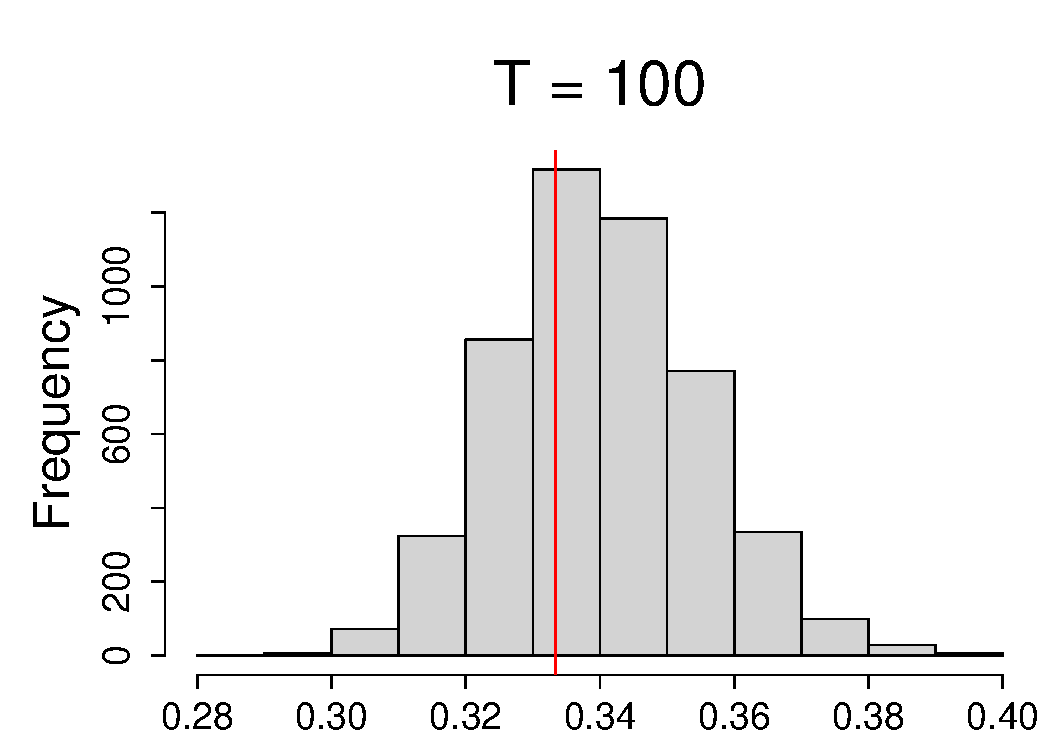
\includegraphics[scale=0.3]{../output/sigma_histogram_zero_function_T_100_b_0.pdf}
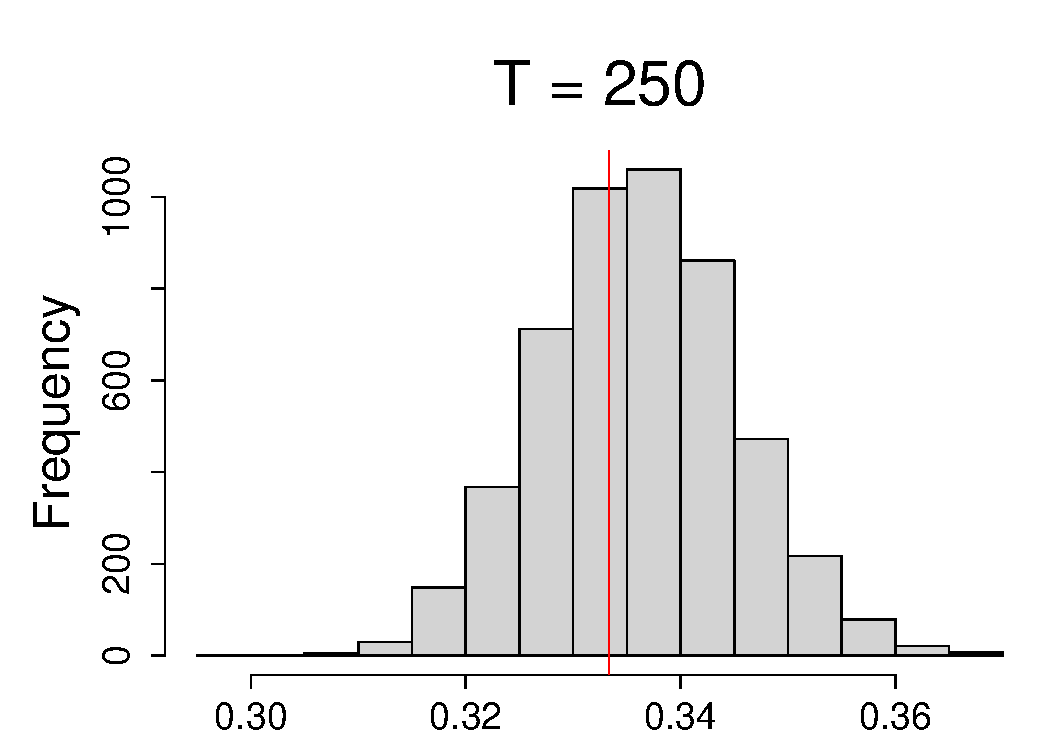
\includegraphics[scale=0.3]{../output/sigma_histogram_zero_function_T_250_b_0.pdf}
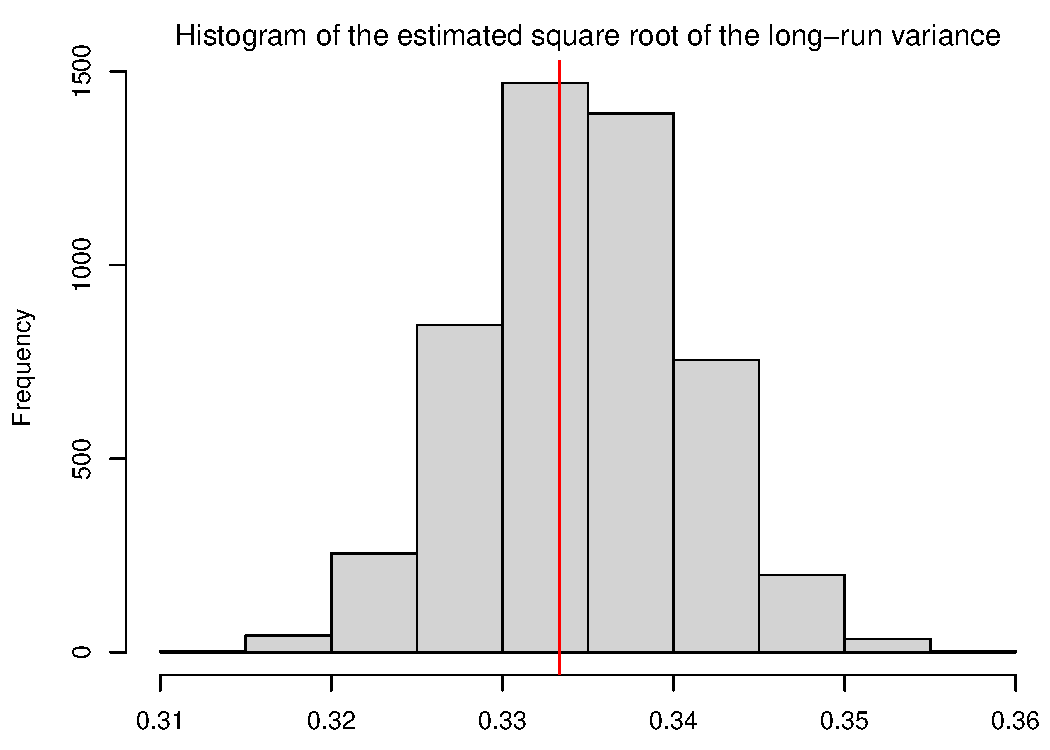
\includegraphics[scale=0.3]{../output/sigma_histogram_zero_function_T_500_b_0.pdf}
\end{subfigure}
\begin{subfigure}[b]{0.4\textwidth}
\centering
\caption{bump function}
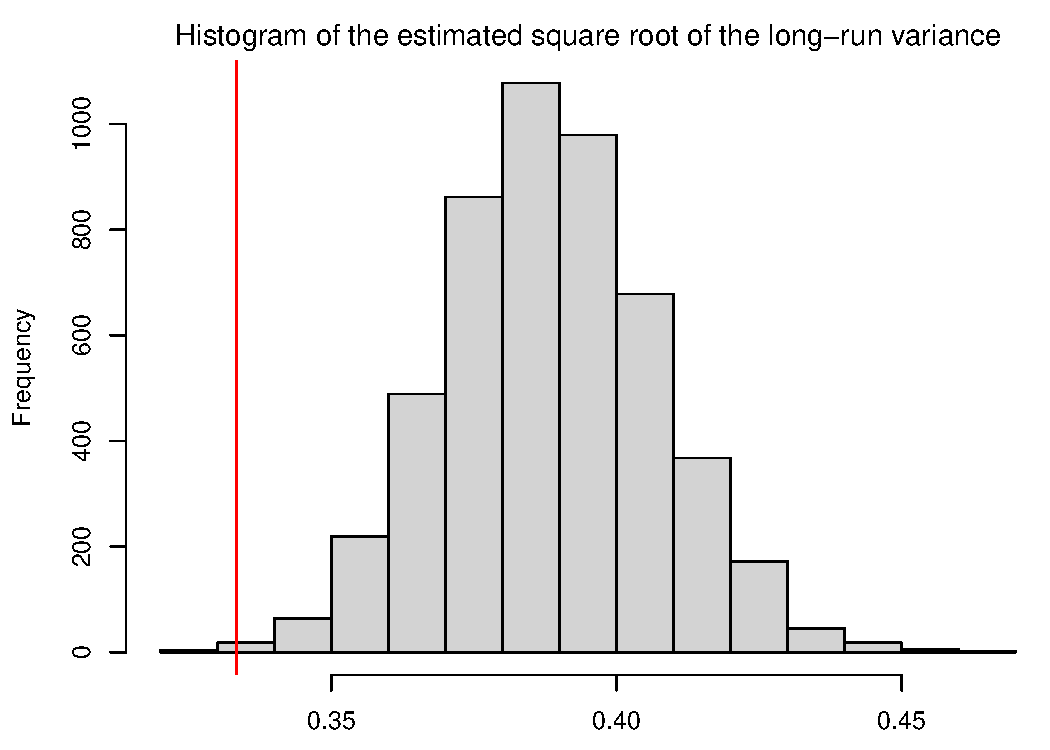
\includegraphics[scale=0.3]{../output/sigma_histogram_bump_function_T_100_b_0.pdf}
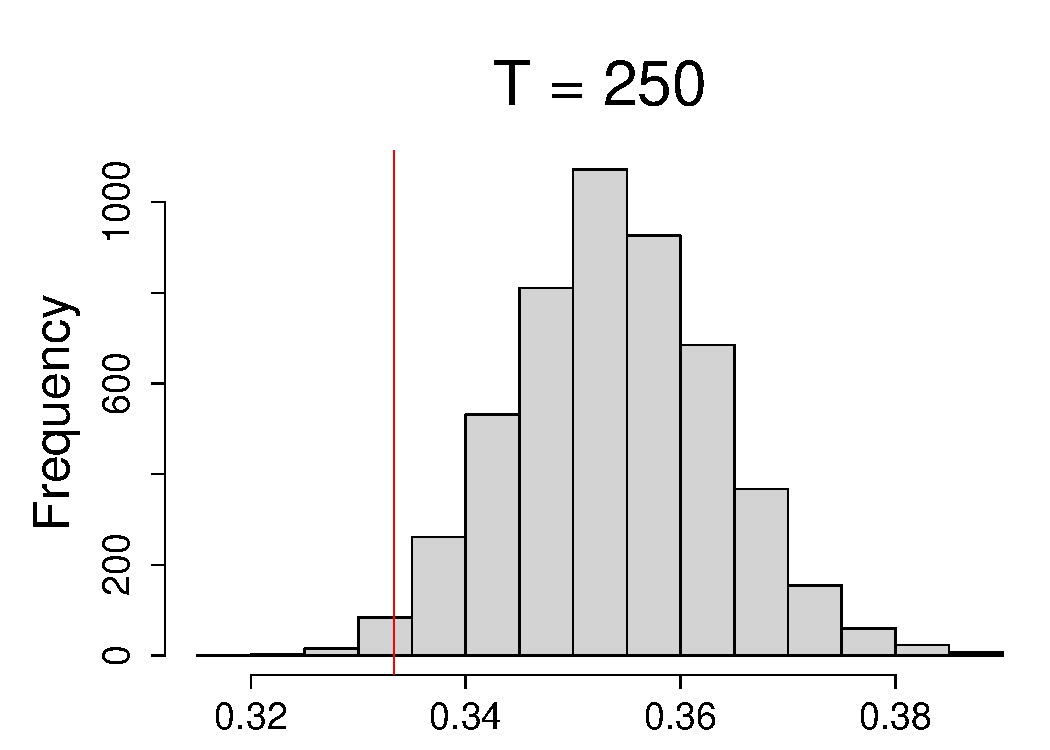
\includegraphics[scale=0.3]{../output/sigma_histogram_bump_function_T_250_b_0.pdf}
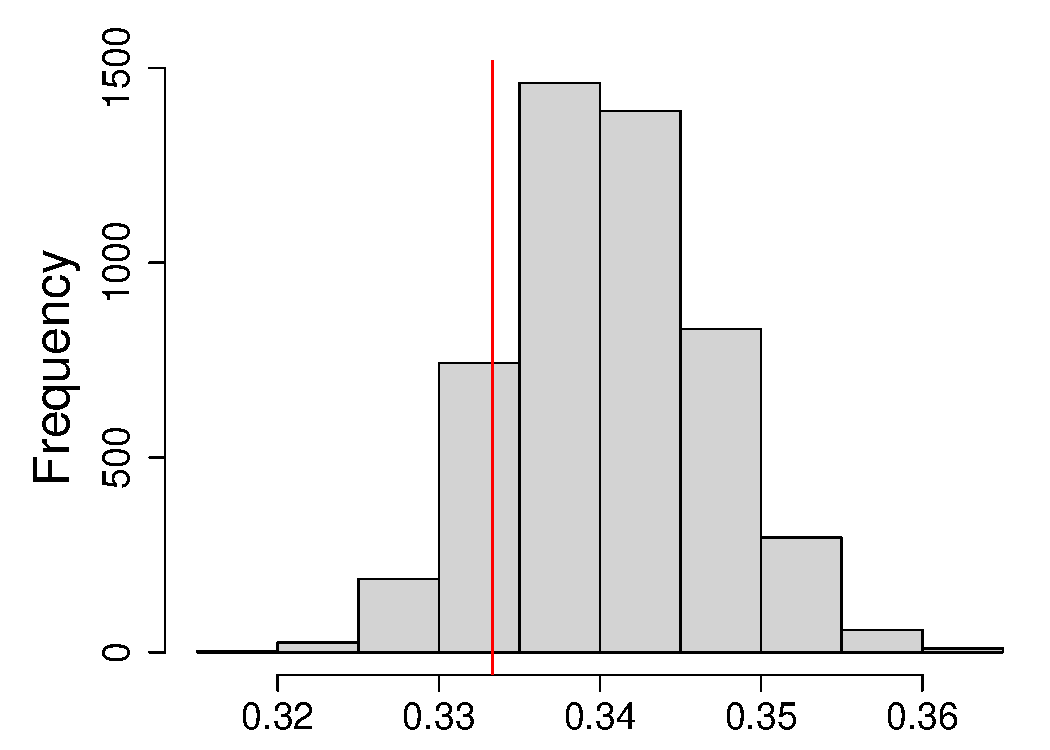
\includegraphics[scale=0.3]{../output/sigma_histogram_bump_function_T_500_b_0.pdf}
\end{subfigure}
\end{figure}

%{\color{red}Marina: The size numbers are a bit more conservative, it seems that the convergence is slower which can be explained by the following. I have also added how precise we are estimating the coefficients and the long-run variance. The results for various sample sizes $T=100, 250, 500$ and two different specifications of the null function (zero functions and bump function as specified above.) are presented in Figures \ref{fig:hist_coefficients:zero} - \ref{fig:hist_lrv:bump}. It is pretty clear that the estimation of he long-run variance is much less precise when we are considering the bump function instead of the zero function. The convergence to the true value as the sample size grows larger is visible but quite slow still.}


\item {\color{black}\textit{I do not understand why the authors are resistant to add the simple competitors suggested (additive models w/ CI-based testing and Bayesian analogs). Their reasoning was 1) these methods do not offer the same theory guarantees and 2) they include another method, sizer, and a simplified version of their approach. For 1): if the theory actually offers practical gains, then this should show up clearly empirically and further advertise the proposed methods! For 2): sizer is a reasonable competitor (for n=2), but I don’t see why that would eliminate consideration of any alternatives. If the question is “which curves are different and when”, a natural first approach would be to fit a nonparametric model to each curve and see where/when the confidence/credible intervals do not overlap (w/ or w/o a Bonferroni correction). Beating this approach will be more convincing for general readers.}}

Following your suggestion, we have added a simple competitor which is based on uniform confidence bands. A detailed description of the competitor and the results of our comparison study can be found in Section A.3 of the supplementary material. The simulation results reported there show that our approach vastly outperforms the competitor.

We have also considered the proposed Bayesian competitor from \cite{Meyer2015} and \cite{Zemplenyi2021}\footnote{We used the code from \url{https://github.com/MorrisStatLab/BayesFMM_Function_on_Function} following \cite{Zemplenyi2021}.} which uses simultaneous band scores (SimBaS). However, at the end of the day, we have not added it to the paper because (in our understanding as non-experts in Bayesian statistics) SimBaS (as implemented in \cite{Meyer2015}) is 
%not an appropriate competitor for our method. 
not fully compatible with our model setting: The model, estimation pipeline, and calibration assumptions of SimBaS all target function-on-function surfaces $\beta(v,t)$ with non-degenerate functional predictors and multiple curves. Forcing the publicly available code to match our setting requires adding jitter or pseudo-replication that changes the estimand and invalidates error control.
%, so any comparison would be methodologically unfair as far as we can see. 
Conceptually, the SimBaS idea may of course be generalized, but that is not what the available code does. 
More specifically, the main issue is this: 
%Specifically, there is an important issue with the mismatch of the target of the analysis. 
As we have understood, SimBaS is defined by inverting joint credible bands over the $2$-D coefficient surface $\beta(v,t)$ for the model $y_{ic}(t) = \int_{v\in V} x_{ic}(v)\beta(v, t)dv + U_i(t) +E_{ic}(t)$ after transforming both $y_{ic}(t)$ and $x_{ic}(v)$ to basis space and standardizing the posterior draws; it then computes $P_{\text{SimBaS}}(v,t)$ using the global maximum over the $(v,t)$ domain (equations (7)--(8) in \cite{Zemplenyi2021}). This controls experiment-wise error across $V\times T$ locations. 
If we want to match this model with ours, we need to assume that $x_{ic}(v) \equiv 1$. 
The problem then collapses to a function-on-scalar coefficient $b(t) := \int_{v\in V} \beta(v, t)dv$, for which the SimBaS surface machinery does not seem to be appropriate. Assuming $x_{ic}(v) \equiv 1$ in particular creates problems in terms of implementation. The WFFR procedure that SimBaS relies on always applies a discrete wavelet transform (DWT) to each row of $\mathbf{X} = \left(x_{ic}(v)\right)_{i, c}$ and then performs wavelet-space PCA before fitting the model. With $x_{ic}(v)\equiv 1$, the DWT of $\mathbf{X}$ is degenerate, the standardization step results in dividing by zero, but the code expects wavelet-spec fields and dimensions that don’t exist in this degenerate case. 
%If we want to match this model with ours, we need to assume that $V=1$ and $x_{ic}(v) \equiv 1$. The problem then collapses to a function-on-scalar coefficient $\beta(t)$, for which the SimBaS surface machinery does not seem to be appropriate. Assuming $V = 1$ and $x_{ic}(v) \equiv 1$ in particular creates problems in terms of implementation. The WFFR procedure that SimBaS relies on always applies a discrete wavelet transform (DWT) to each row of $\mathbf{X} = \left(x_{ic}(t)\right)_{i, c}$ and then performs wavelet-space PCA before fitting the model. With $x_{ic}(v)\equiv 1$ or $V=1$, the DWT of $\mathbf{X}$ is degenerate, the standardization step results in dividing by zero, but the code expects wavelet-spec fields and dimensions that don’t exist in this degenerate case. 
%\textcolor{red}{[I guess this is enough and we can skip the following: 
%Another issue is that SimBaS calibration presumes multiple curves ($N\geq 2$) and can not be applied for each time series separately. Posterior credible bands and their maxima used for calculating $P_{\text{SimBaS}}(v, t)$ rely on estimating residual variance and random-effect variability that require information from more than one curve; otherwise, posterior inferences for $\beta(v, t)$ and, crucially, the band widths used by SimBaS hinge almost entirely on the prior rather than data. This is why the simulations and application in \cite{Zemplenyi2021} use nontrivial sample sizes (e.g., $N=25$ with repeated measures and larger), and they report performance improving as sample size increases.]} \\
In summary, (as non-experts in Bayesian statistics) we believe that as currently implemented, SimBaS is not compatible with our model setting and thus cannot be regarded as an off-the-shelf benchmark. For this reason, we have not considered it in the revision. 
%SimBaS is not a suitable competitor for our method, and that adapting it to our setting would constitute a new method, not an off-the-shelf benchmark.

%{\color{red}
%Not sure whether the proposed matching with $V=1$ and $x_{ic}(v) \equiv 1$ is correct: 
%\begin{itemize}
%\item By $V=1$, I guess you mean $V = \{1\}$, or more precisely, $V$ a set that consists of exactly one point. If so, then the integral $\int_{v \in V}$ becomes degenerate, i.e., $\int_{v\in V} x_{ic}(v)\beta(v, t)dv \equiv 0$. To match the model with ours, I guess it is enough to set $x_{ic}(v) \equiv 1$. Then $\int_{v\in V} x_{ic}(v)\beta(v, t)dv = b(t)$, i.e., we have reduced everything to a function-on-scalar coefficient $b(t)$. Isn't that right? \textcolor{blue}{$V$ is the length of the grid $\mathbf{v} = [v_1, \ldots, v_V]$ where $x_{ic}(v)$ is observed and I agree that in terms of the integral it becomes a degenerate one. However, they also have a discretized version of the model, $\mathbf{y}_{ic} = \mathbf{x}_{ic} \bfbeta \Delta_{v_j} + \mathbf{u}_i + \mathbf{e}_{ic}$, where $\mathbf{y}_{ic}$, $\mathbf{u}_i$, $\mathbf{e}_{ic}$ are $1\times T$, $\mathbf{x}_{ic}$ is $1\times V$, $\Delta_{v_j} = v_j - v_{j-1}$ and $\bfbeta$ is $V\times T$. They further work with this discretized version which by the way does not include $\alpha(t)$ at all because "in practice, we center both $y_{ic}(t)$ and $x_{ic}(v)$ and thus, without loss of generality, $\alpha(t)$ in Model 1 (with integral) is zero and not needed in Model 2 (discretized)". This also answers your next question that there are no credible bands for $\alpha(t)$. And yes, I have tried to set $x_{ic}(v) \equiv 1$ but this is exactly what is not supported in the code: it tries to do PCA (which is not the problem since I can circumvent it) and some wavelet transformation (which is the problem) on $x_{ic}$ which requires some variance of the curves.} 
%\item Another point of view: Couldn't one match the model with ours by simply setting $x_{ic}(v) \equiv 0$, which leads to $y_{ic}(t) = \alpha(t) + U_i(t) +E_{ic}(t)$? In this model, $ \alpha(t)$ is the common trend. Or does SimBaS provide credible bands only for the component $\int_{v\in V} x_{ic}(v)\beta(v, t)dv$ but not for $\alpha(t)$?
%\end{itemize}
%Finally two questions: $x_{ic}$ are observed time-independent covariates (or more specifically, covariate processes in $v$), correct? \textcolor{blue}{Exactly, the covariates do not depend on $t$, only on $v$.} What is the subscript $c$ in the notation? \textcolor{blue}{The subscript $c$ denotes repeated measurements for a subject $i$: $c = 1, \ldots, C_i$. I guess for us that means that $C_i$ = 1 for all $i$. By the way, $N$ from above is equal to the total number of curves, i.e., $N= \sum_{i=1}^n C_i$.}
%}
 
%We have added the following naive competitor that is based on the uniform confidence bands (UCB) based from \cite{Kim2016}:

%\begin{itemize}
%\item We consider the model without the fixed effects $\alpha_i$ since the specification in \cite{Kim2016} does not allow for fixed effects.
%\item For each of the time series $i = 1, \ldots, n$, we calculate the UCB as described in \cite{Kim2016} using bandwidth $0.2$. {\color{red}Marina: optimal bandwidth using cross-validation was not that easy to calculate and the theoretical optimal bandwidths were $0.4, 0.33, 0.29$ for $T=100, 250, 500$, respectively.}
%\item For each pairwise comparison $(i, j)$, we consider the null hypothesis rejected if there is $t \in \{1, \ldots, T\}$ with a condition that $t/T \in [0.05, 0.95]$ (since the estimation procedure proposed in \cite{Kim2016} has poor performance at the boundaries, we have decided to exclude them from analysis) such that the UCBs for $m_i(t/T)$ and $m_j(t/T)$ do not overlap.
%\item We do not apply any correction for the multiple testing problem.
%\item We consider $\alpha = 0.05$.
%\item We calculate how many times we reject the null for this naive competitor. The results are presented in Table \ref{tab:sizepower_UCB}. {\color{red} Marina: we are reporting here the global power for the competitor which is not super comparable to the other types of power that we have. On the other hand, even this power is still worse than our actual power. What do you think?}
%\end{itemize}

%For the smallest sampel size $T=100$, the UCBs for two trend functions remain relatively wide compared to the strength of the signal so that we almost never detect any differences. For larger sample sizes ($T=250, 500$), this naive compatitor is able to detect the differences for the strong sygnal. However, we should point out that we did not account for multiple testing here and we expect that with Bonferroni correction, the UCBs will become much wider so that even the strongest will not be detectable. 

%Examples of two UCBs for $T=500$ and different values of $b$ are presented in Figure \ref{fig:UCB}.


\item {\color{black}\textit{Stochastic volatility (SV) is widely important in the types of applications that the authors mention. Yet the authors 1) claim that extensions to SV would be challenging, 2) elect not to consider any simulation designs with SV to examine robustness, and 3) claim that SV can be handled with log-transformations (and then using the same mean models as proposed). Perhaps 1) is true, but 2) is important based on the claims in the paper and the relevance for this journal. Finally, 3) is not correct for the most widely-used SV models.}}

With stochastic volatility, we guess you mean time-varying (short-run and long-run) error variance.

ad 2) As a robustness check, we have included a design with time-varying error variance in the revised simulation study. More specifically, we assume that for each $i$, the idiosyncratic error process $\{\varepsilon_{it}: 1 \le t \le T\}$ follows an AR(1) model with a time-varying (short- and long-run) variance. The details can be found in Section A.2.4 of the supplement. 

%we assume that for each $i$, the idiosyncratic error process $\{\varepsilon_{it}: 1 \le t \le T\}$ follows the AR(1) model $\varepsilon_{it} = a \varepsilon_{i t-1} + \sigma(t/T)\eta_{it}$, where $a = 0.25$, the innovations $\eta_{it}$ are i.i.d.\ normally distributed with mean $0$ and standard deviation $1$ and $\sigma^2(u) = -\frac{3}{8}(x-0.5)^2 + \frac{3}{32}$ for $u \in [0, 1]$ (see also Figure \ref{fig:SV_plot} for $T=500$). The choice of the coefficients is driven by the requirement $\int_0^1 \sigma^2(u)du = 0.25^2$ that was introduced so that this simulation scenario is comparable to the ones with constant variance. The calculation of the critical values is also performed using the time-varying variance. All of the other parameters of the DGP remain the same. The results are presented in Tables \ref{tab:size_SV} - \ref{tab:fullpower_SV}.

ad 3) We fully agree that log-transformations only work in special cases. We mentioned them in our reply letter to your previous referee report only to point out that at least in some special cases, our methods can easily accommodate time-varying error variances. 


\end{enumerate}



\subsection*{Reply to referee 2}


Thank you very much for the careful reading of our manuscript. We have addressed your remaining question in the revision. Please see our reply below.
\begin{enumerate}[label=\arabic*.,leftmargin=0.6cm]
  
\item \textit{Thank you very much for your very careful revision. I have just one remaining "cosmetic" question: can you explain why in the third row of your figures such as Figure 1, page 27, we see several intervals one on top of the other? In other words is there a meaning of the y-axis of this lower plots, what is its scale? Thank you in advance for adding this information (which I might have missed elsewhere?).}

The third row of our figures (such as Figure 1) shows the intervals that are contained in the sets $\mathcal{S}^{[i, j]}(\alpha)$. To make these intervals all visible, we plot them one on top of the other. However, the order in which we plot them is completely arbitrary, i.e., their vertical positioning does not contain any information. We have clarified this in the figure caption.

\end{enumerate}



\bibliographystyle{ims}
{\small
\setlength{\bibsep}{0.55em}
\bibliography{bib}



\end{document}
